
\chapter{Neymanian Repeated Sampling Inference in Completely Randomized Experiments}\label{chapter::neyman-cr}
 \chaptermark{Completely Randomized Experiment and Neymanian Inference}
 
 
In his seminal paper,  \citet{Neyman:1923} not only proposed the notation of potential outcomes but also derived rigorous mathematical results for making inference for the average causal effect under a CRE. In contrast to Fisher's idea of calculating the $p$-value under the sharp null hypothesis, \citet{Neyman:1923} proposed an unbiased point estimator and a conservative confidence interval based on the sampling distribution of the point estimator. This chapter will introduce \citet{Neyman:1923}'s fundamental results, which are very important for understanding later chapters in Part \ref{part::rcts} of this book.



\section{Finite population quantities}

Consider a CRE with $n$ units, where $n_1$ of them receive the treatment and $n_0$ of them receive the control. For unit $i = 1, \ldots, n$, we have potential outcomes $Y_i(1)$ and $Y_i(0)$, and individual effect $\tau_i = Y_i(1) - Y_i(0).$ The potential outcomes have finite population means  
$$
\bar{Y}(1) = n^{-1} \sumn Y_i(1),\quad
\bar{Y}(0) = n^{-1} \sumn Y_i(0),
$$
variances\footnote{Here the divisor $n-1$ makes the main theorems in this chapter more elegant. Changing the divisor to $n$ complicates the formulas but does not change the results fundamentally. With large $n$, the difference is minor.}
$$
S^2(1) = (n-1)^{-1} \sumn \{ Y_i(1) -\bar{Y}(1)  \}^2,\quad
S^2(0) = (n-1)^{-1} \sumn \{ Y_i(0) -\bar{Y}(0)  \}^2 ,
$$
and covariance
$$
S(1,0) = (n-1)^{-1} \sumn \{ Y_i(1) -\bar{Y}(1)  \}\{ Y_i(0) -\bar{Y}(0)  \} . 
$$
The individual effects have mean
$$
\tau = n^{-1} \sumn \tau_i = \bar{Y}(1) - \bar{Y}(0) .
$$
and variance
$$
S^2(\tau) = (n-1)^{-1} \sumn (\tau_i - \tau)^2.
$$
We have the following relationship between the variances and covariance.
\begin{lemma}\label{lemma::variancecovariancetau}
$2S(1,0) = S^2(1)+S^2(0) - S^2(\tau).$
\end{lemma}

Lemma \ref{lemma::variancecovariancetau}  is a basic result and will be useful for later discussion. 
The proof of Lemma \ref{lemma::variancecovariancetau} follows from elementary algebra. I leave it as Problem \ref{hw::proof-covariance-basic}. 

These fixed quantities are functions of the Science Table $\{ Y_i(1), Y_i(0)  \}_{i=1}^n$. We are interested in estimating the average causal effect $\tau$ based on the data $ (Z_i, Y_i)_{i=1}^n$ from a CRE. 


\section{\citet{Neyman:1923}'s theorem}


Based on the observed outcomes, we can calculate the sample means
$$
\hat{\bar{Y}}(1) = n_1^{-1} \sumn Z_i Y_i,\quad
\hat{\bar{Y}}(0) = n_0^{-1} \sumn (1-Z_i) Y_i,
$$
the sample variances
$$
\hat{S}^2(1) = (n_1 - 1)^{-1} \sumn Z_i  \{  Y_i - \hat{\bar{Y}}(1) \}^2,\quad
\hat{S}^2(0) = (n_0 - 1)^{-1} \sumn (1-Z_i)  \{  Y_i - \hat{\bar{Y}}(0) \}^2 . 
$$
But there are no sample versions of $S(1,0)$ and $S^2(\tau)$ because the potential outcomes $Y_i(1)$ and $Y_i(0)$ are never jointly observed for each unit $i$. \citet{Neyman:1923} proved the following theorem. 




\begin{theorem}
\label{thm::neyman1923}
Under a CRE, 
\begin{enumerate}
\item
the difference-in-means estimator $\hat{\tau} =\hat{\bar{Y}}(1) -  \hat{\bar{Y}}(0)$ is unbiased for $\tau$:
$$
E(\hat{\tau}) =\tau ;
$$ 
\item
$\hat{\tau} $ has variance 
\begin{eqnarray}
\var(\hat{\tau})  &=&  \frac{S^2(1)}{n_1} + \frac{S^2(0)}{n_0} - \frac{S^2(\tau)}{n} \label{eq::neyman23var} \\
&=& \frac{n_0}{n_1 n} S^2(1) + \frac{n_1}{n_0 n} S^2(0) + \frac{2}{n} S(1,0) ;  \label{eq::neyman23var-equivalent}
\end{eqnarray}
\item\label{neyman-3}
the variance estimator 
$$
\hat{V} = \frac{\hat{S}^2(1)}{n_1} + \frac{\hat{S}^2(0)}{n_0}
$$
is conservative for estimating $\var(\hat{\tau})$ in the sense that 
$$
E(\hat{V} ) - \var(\hat{\tau})  = \frac{S^2(\tau)}{n}  \geq 0
$$
with equality holding if and only if $\tau_i = \tau$ for all units. 
\end{enumerate}
\end{theorem}

I will present the proof of Theorem \ref{thm::neyman1923} in Section \ref{sec::prove-neyman-1923}. Before proving Theorem \ref{thm::neyman1923},  it is important to clarify the meanings of $E(\cdot)$ and $\var(\cdot)$ in Theorem \ref{thm::neyman1923}. The potential outcomes are all fixed numbers, and only the treatment indicators $Z_i$'s are random. Therefore, the expectations and variances are all over the randomness of the $Z_i$'s, which are random permutations of $n_1$ 1's and $n_0$ 0's. Figure \ref{fig::neyman1923} illustrates the randomness of $\hat\tau$, which is a discrete uniform distribution over $\{ \hat\tau^1 , \ldots, \hat\tau^M\}$ induced by  $M=\binom{n}{n_1}$ possible treatment allocations. 
Compare Figure \ref{fig::neyman1923} with Figure \ref{fig::frt} to see the key differences between the FRT and \citet{Neyman:1923}'s theorem:
\begin{enumerate}
\item
The FRT works for any test statistic but \citet{Neyman:1923}'s theorem is only about the difference in means. Although we could derive the properties of other estimators similar to \citet{Neyman:1923}'s theorem,  this mathematical exercise is often quite challenging for general estimators. 

\item
In Figure \ref{fig::frt}, the observed outcome vector $\bm{Y}$ is fixed but in Figure \ref{fig::neyman1923}, the observed outcome vector $\bm{Y}(\bm{z}^m)$ changes as $\bm{z}^m$ changes. 

\item
The $T(\bm{z}^m,\bm{Y}) $'s In Figure \ref{fig::frt} are all computable based on the observed data, but the $\hat\tau^m$'s in Figure \ref{fig::neyman1923} are hypothetical values because not all potential outcomes are known. 
\end{enumerate}

\begin{figure}[ht]
\centering 
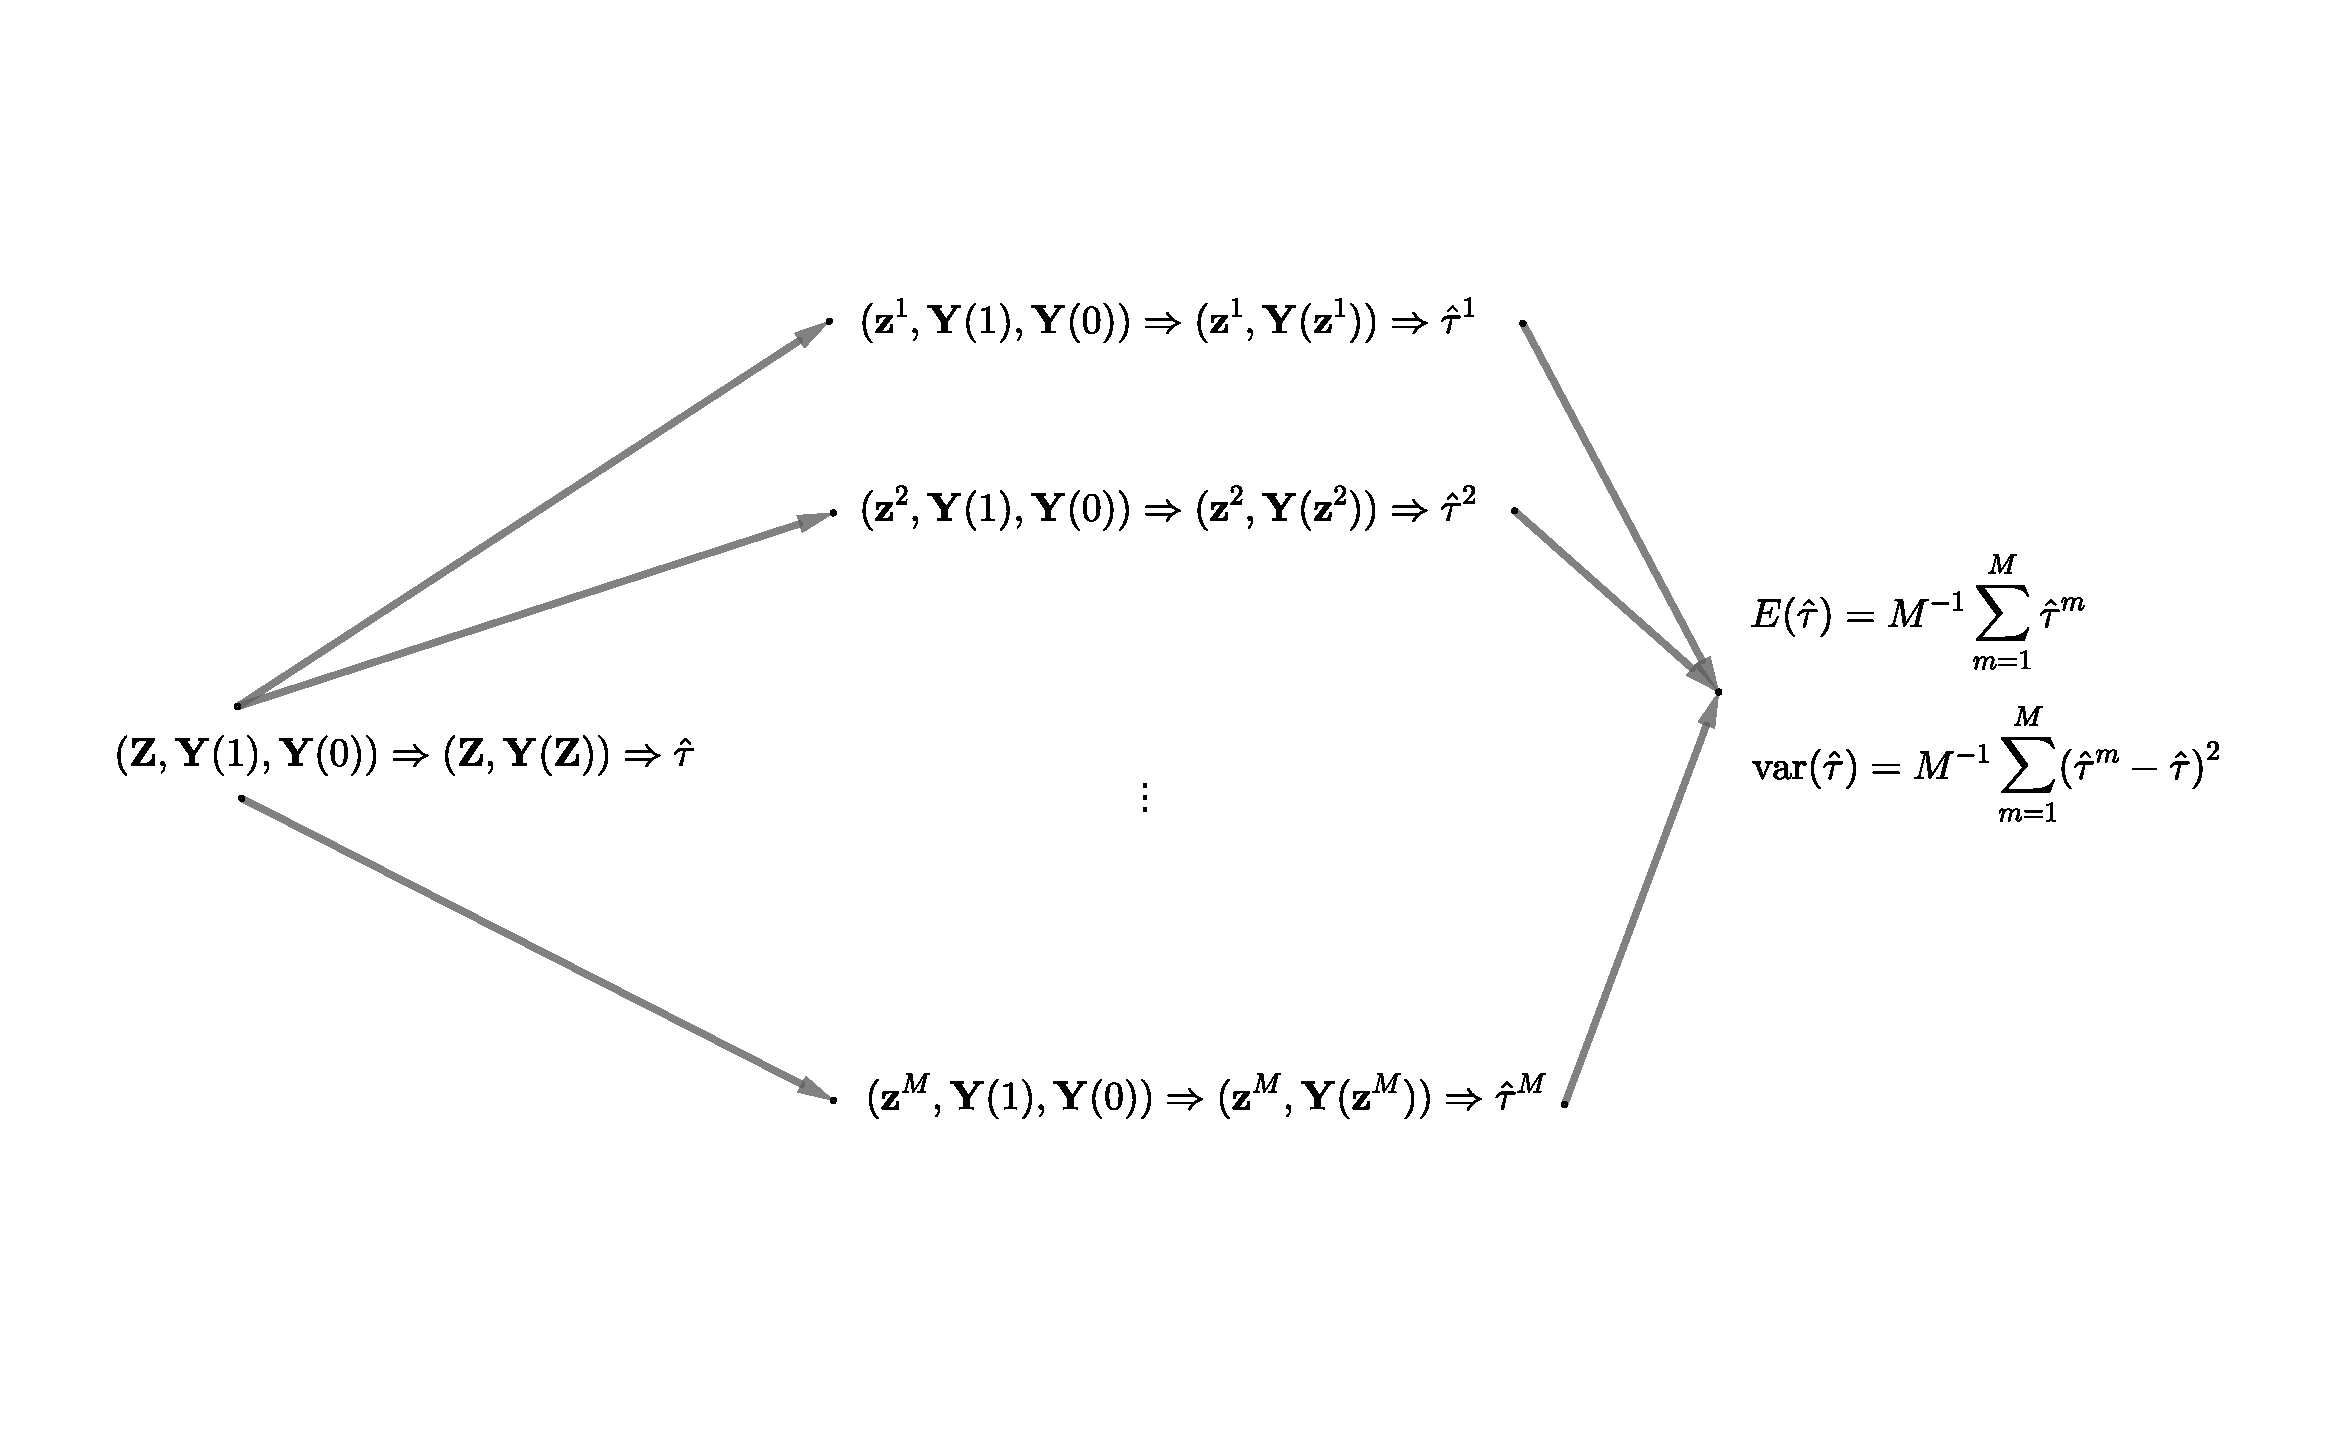
\includegraphics[width =  \textwidth]{figures/neyman1923_fig.pdf}
\caption{Illustration of \citet{Neyman:1923}'s theorem, where $\bm{Y}(\bm{z}^m)$ is the observed outcome vector under the treatment vector $\bm{z}^m$.}\label{fig::neyman1923}
\end{figure}




The point estimator $\hat\tau$ is standard but it has a non-trivial variance under the potential outcomes framework with a CRE. The variance formula \eqref{eq::neyman23var} differs from the classic variance formula for the difference in means\footnote{In the classic two-sample problem, the outcomes under the treatment are IID draws from a distribution with mean $\mu_1$ and variance $\sigma_1^2$, and the outcomes under the control are IID draws from a distribution with mean $\mu_0$ and variance $\sigma_0^2$. Under this assumption, we have 
$$
\var(\hat{\tau} ) = \frac{\sigma_1^2}{n_1} +  \frac{\sigma_0^2}{n_0}.
$$
Here, $\var(\cdot)$ is over the randomness of the outcomes. This variance formula does not involve a third term that depends on the variance of the individual causal effects. 
} because it not only depends on the finite population variances of the potential outcomes but also depends on the finite population variance of the individual effects, or, equivalently, the finite population covariance of the potential outcomes. Unfortunately, $S^2(\tau)$ and $S(1,0)$ are not identifiable from the data because  $Y_i(1)$ and $Y_i(0)$ are never jointly observed. 




The formula \eqref{eq::neyman23var} is a little puzzling in that the more heterogeneous the individual effects are the smaller the variability of $\hat{\tau}$ is. Section \ref{sec::simulation-neyman-formula} will use numerical examples to verify \eqref{eq::neyman23var}. What is the intuition here? I give an explanation based on the equivalent form \eqref{eq::neyman23var-equivalent}. Compare the case with positively correlated potential outcomes and the case with negatively correlated potential outcomes. 
Although the treatment group is a simple random sample from the finite population of $n$ units, it is possible to observe relatively large treatment potential outcomes in a realized experiment. Assume this happens. 
\begin{enumerate}
\item
If $S(1,0) > 0$, then those treated units also have relatively large control potential outcomes. Consequently, the observed outcomes under control are relatively small, which results in large $\hat\tau$. 
\item
If $S(1,0) < 0$, then those treated units have relatively small control potential outcomes. Consequently, the observed outcomes under control are relatively large, which results in small $\hat\tau$. 
\end{enumerate}
The reverse can also happen if we observe relatively small treatment potential outcomes in a realized experiment. Overall, although the unbiasedness of $\hat\tau$ does not depend on the correlation between the potential outcomes,  it is more likely to observe more extreme $\hat\tau$ under $S(1,0) > 0$ than under $S(1,0) < 0$. So the variance of $\hat{\tau}$ is larger when the potential outcomes are positively correlated. 

 
 
 
 


\citet[][Theorem 5 and Proposition 3]{li2017general} further proved the following asymptotic Normality of $\hat{\tau}$ based on the finite population CLT.
\begin{theorem}
\label{thm::clt-difference-in-means}
Let $n\rightarrow \infty$ and $n_1 \rightarrow \infty$. 
If $n_1/n$ has a limiting value in $(0,1)$,  $\{S^2(1), S^2(0), S(1,0)\}$ have limiting values, and 
$$  
\max_{1\leq i \leq n}\{ Y_i(1) - \bar{Y}(1) \}^2/n \rightarrow 0, \quad 
\max_{1\leq i \leq n}\{ Y_i(0) - \bar{Y}(0) \}^2/n \rightarrow 0,
$$
then 
$$
\frac{   \hat{\tau} - \tau }{  \sqrt{ \var(\hat{\tau}) } } \rightarrow \N01
$$
in distribution, and
$$
\hat{S}^2(1) \rightarrow S^2(1),\quad 
\hat{S}^2(0) \rightarrow S^2(0)
$$
in probability. 
\end{theorem}


The proof of  Theorem \ref{thm::clt-difference-in-means} is technical and beyond the scope of this book. It ensures that the sampling distribution of $\hat{\tau} $ can be approximated by a Normal distribution with a large sample size and some regularity conditions. Moreover, it ensures that the sample variances of the outcomes are consistent for the population variances, which further ensures that the probability limit of \cite{Neyman:1923}'s variance estimator is larger than the true variance of $\hat{\tau} $. This justifies a conservative large-sample confidence interval for $\tau$: 
$$
\hat{\tau} \pm z_{1-\alpha/2} \sqrt{  \hat{V}  },
$$
where $z_{1-\alpha/2}$ is the $1-\alpha/2$ upper quantile of the standard Normal random variable. It is the same as the confidence interval for the standard two-sample problem asymptotically (see Chapter \ref{sec::bf-problem}). This confidence interval covers $\tau$ with probability at least as large as $1-\alpha$ when the sample size is large enough. By duality, the confidence interval implies a test for 
$$
\HN: \tau = 0,
$$
which is called the weak null hypothesis. 



Due to the fundamental problem of missing one potential outcome, we can at most obtain a conservative variance estimator. In statistics, the definition of the confidence interval allows for over coverage and thus conservativeness in variance estimation (see Chapter \ref{sec::statistical-inference}).  Conservativeness is not a big problem if underreporting the treatment effect is not a big problem in practice. Sometimes, it can be problematic if the outcomes measure the side effects of a treatment. In medical experiments, underreporting the side effects of a new drug can have severe consequences on patients' health. 
 
 

\section{Proofs}\label{sec::prove-neyman-1923}

In this section, I will prove  Theorem \ref{thm::neyman1923}.


First, the unbiasedness of $\hat{\tau}$ follows from the representation
\begin{eqnarray*}
\hat{\tau} &=& n_1^{-1} \sumn Z_i Y_i - n_0^{-1} \sumn (1-Z_i) Y_i \\
&=& n_1^{-1} \sumn Z_i Y_i(1) - n_0^{-1} \sumn (1-Z_i) Y_i(0) 
\end{eqnarray*}
and the linearity of the expectation:
\begin{eqnarray*}
E( \hat{\tau}  ) &=& E\left\{    n_1^{-1} \sumn Z_i Y_i(1) - n_0^{-1} \sumn (1-Z_i) Y_i(0)   \right\} \\
&=& n_1^{-1} \sumn E(Z_i) Y_i(1) - n_0^{-1} \sumn E(1-Z_i) Y_i(0) \\
&=& n_1^{-1} \sumn \frac{n_1}{n} Y_i(1) - n_0^{-1} \sumn \frac{n_0}{n} Y_i(0) \\
&=&  n^{-1} \sumn Y_i(1) - n^{-1} \sumn Y_i(0) \\
&=& \tau .
\end{eqnarray*}


Second, we can further write $\hat{\tau}$ as
\begin{eqnarray*}
\hat{\tau} &=&  \sumn Z_i  \left\{    \frac{  Y_i(1) }{ n_1 } + \frac{  Y_i(0) }{ n_0 }   \right\}
- n_0^{-1} \sumn Y_i(0).
\end{eqnarray*}
The variance of $\hat{\tau}$ follows from Lemma \ref{lemma::samplemean} of simple random sampling:
\begin{eqnarray*}
\var(\hat{\tau}) &=&  \frac{  n_1 n_0  }{  n(n-1)  }  \sumn  
\left\{    \frac{  Y_i(1) }{ n_1 } + \frac{  Y_i(0) }{ n_0 }  -  \frac{  \bar{Y}(1) }{ n_1 } - \frac{  \bar{Y}(0) }{ n_0 }    \right\}^2 \\
&=&  \frac{  n_1 n_0  }{  n(n-1)  }  \left[
\frac{1}{n_1^{2}}   \sumn  \{  Y_i(1) -  \bar{Y}(1)\}^2 + \frac{1}{n_0^{2}}  \sumn  \{  Y_i(0) -  \bar{Y}(0)\}^2 \right. \\
&& \left. \qquad \qquad 
+ \frac{2}{n_1 n_0}  \sumn  \{  Y_i(1) -  \bar{Y}(1)\}  \{  Y_i(0) -  \bar{Y}(0)\} 
\right]\\
&=& \frac{n_0}{n_1n} S^2(1) + \frac{n_1}{n_0n}S^2(0) + \frac{2}{n} S(1,0). 
\end{eqnarray*}
From Lemma \ref{lemma::variancecovariancetau}, we can also write the variance as
\begin{eqnarray*}
\var(\hat{\tau})
&=& \frac{n_0}{n_1n} S^2(1) + \frac{n_1}{n_0n}S^2(0) + \frac{1}{n} \{ S^2(1)+S^2(0) - S^2(\tau) \}\\
&=&  \frac{S^2(1)}{n_1} + \frac{S^2(0)}{n_0} - \frac{S^2(\tau)}{n}.
\end{eqnarray*}

Third, because the treatment group is a simple random sample of size $n_1$ from the $n$ units, Lemma \ref{lemma::variance-unbiased} ensures that the sample variance of $Y_i(1)$'s is unbiased for its population variance: 
$$
E\{  \hat{S}^2(1) \} = S^2(1).
$$
Similarly, $E\{  \hat{S}^2(0) \} = S^2(0).$ Therefore, $\hat{V} $ is unbiased for the first two terms in \eqref{eq::neyman23var}. 
 
 
 
 
 \section{Regression analysis of the CRE}
 
 
 
Practitioners often use regression-based inference for the average causal effect $\tau$. A standard approach is to run the ordinary least squares (OLS) of the outcomes on the treatment indicators with an intercept
$$
(\hat\alpha, \hat\beta) = \arg\min_{(a,b)} \sum_{i=1}^n (Y_i - a - bZ_i)^2,
$$
and use the coefficient of the treatment $ \hat\beta$ as the estimator for the average causal effect. 
We can show the coefficient $ \hat\beta$  equals the difference in means:
\begin{equation}
\label{eq::ols-difference-in-means}
\hat\beta = \hat\tau .
\end{equation}

However, the usual variance estimator from the OLS (see \eqref{eq::v-hat-ols} in Chapter \ref{appendix::basic-linear-regression}), e.g., the output from the \ri{lm} function of \ri{R}, equals
\begin{eqnarray}
\label{eq::ols-se}
\hat V_\textsc{ols} &=& \frac{n\left(n_1 -1\right)}{( n-2 ) n_1  n_0 } \hat S^2(1) +\frac{n\left(n_0 -1\right)}{( n-2 ) n_1  n_0 } \hat S^2(0)\\
\nonumber &\approx& \frac{\hat S^2(1)}{n_0 }+\frac{ \hat S^2(0) }{n_1 },
\end{eqnarray}
where the approximation holds with large $ n_1 $ and $ n_0 $. It differs from $\hat{V}$ even with large $ n_1 $ and $ n_0 $. 


Fortunately, the Eicker--Huber--White (EHW) robust variance estimator (see \eqref{eq::v-hat-ehw} in Chapter \ref{appendix::basic-linear-regression}) is close to $\hat{V}$:
 \begin{eqnarray}
\label{eq::ols-ehw}
\hat V_\textsc{ehw} &=& \frac{\hat S^2(1)}{n_1 } \frac{n_1 -1}{n_1 }+\frac{\hat S^2(0)}{n_0 } \frac{n_0 -1}{n_0 } \\
\nonumber &\approx& \frac{ \hat S^2(1)  }{n_1 }+\frac{ \hat S^2(0) }{n_0 }
\end{eqnarray}
where the approximation holds with large $ n_1 $ and $ n_0 $. It is almost identical to $\hat{V}$. Moreover, the so-called HC2 variant of the EHW robust variance estimator is identical to  $\hat{V}$. The \ri{hccm} function in the \ri{car} package returns the EHW robust variance estimator as well as its HC2 variant. 

Problem \ref{hw::neyman-ols-nox} provides more technical details for \eqref{eq::ols-difference-in-means}--\eqref{eq::ols-ehw}. 
 



 

 
\section{Examples} 


\subsection{Simulation}
\label{sec::simulation-neyman-formula}



I first choose the sample size as $n=100$ with $60$ treated and $40$ control units, and generate the potential outcomes with constant individual causal effects. 
\begin{lstlisting}
n  = 100
n1 = 60
n0 = 40
y0 = rexp(n)
y0 = sort(y0, decreasing = TRUE)
y1 = y0 + 1
 \end{lstlisting}
With the Science Table fixed, I repeatedly generate CREs and apply Theorem \ref{thm::neyman1923} to obtain the point estimator, the conservative variance estimator, and the confidence interval based on the Normal approximation. 
The $(1,1)$th panel of Figure \ref{fig::simulation-neyman} shows the scatter plot of the potential outcomes,
and the $(1,2)$th panel of Figure \ref{fig::simulation-neyman}  shows the histogram of $\hat{\tau} - \tau$. 

I then change the potential outcomes by sorting the control potential outcomes in reverse order
\begin{lstlisting}
y0 = sort(y0, decreasing = FALSE)
 \end{lstlisting}
and repeat the above simulation. 
The $(2,1)$th panel of Figure \ref{fig::simulation-neyman} shows the scatter plot of the potential outcomes,
and the $(2,2)$th panel of Figure \ref{fig::simulation-neyman}  shows the histogram of $\hat{\tau} - \tau$. 




I finally permute the control potential outcomes randomly 
 \begin{lstlisting}
y0 = sample(y0)
 \end{lstlisting}
 and repeat the above simulation. 
 The $(3,1)$th panel of Figure \ref{fig::simulation-neyman} shows the scatter plot of the potential outcomes,
and the $(2,2)$th panel of Figure \ref{fig::simulation-neyman}  shows the histogram of $\hat{\tau} - \tau$. 

 
 Importantly, in the above three sets of simulations, the correlations between potential outcomes are different but the marginal distributions are the same. The following table compares the true variances, the average estimated variances, and the coverage rates of the $95\%$ confidence intervals. 
 \begin{lstlisting}
              constant negative independent
var              0.036    0.007       0.020
estimated var    0.036    0.036       0.036
coverege rate    0.947    1.000       0.989
 \end{lstlisting}
The true variance depends on the correlation between the potential outcomes, with positively correlated potential outcomes corresponding to a larger sampling variance. This verifies \eqref{eq::neyman23var-equivalent}. The estimated variances are almost identical because the formula of $\hat{V}$ depends only on the marginal distributions of the potential outcomes. Due to the discrepancy between the true and estimated variances, the coverage rates differ across the three sets of simulations. Only with constant causal effects, the estimated variance is identical to the true variance, verifying point \ref{neyman-3} of Theorem \ref{thm::neyman1923}. 
 
Figure \ref{fig::simulation-neyman} also shows the Normal density curves based on the CLT for $\hat{\tau} $. They are very close to the histogram over simulations, verifying Theorem \ref{thm::clt-difference-in-means}.
 
 
 \begin{figure}
 \centering 
 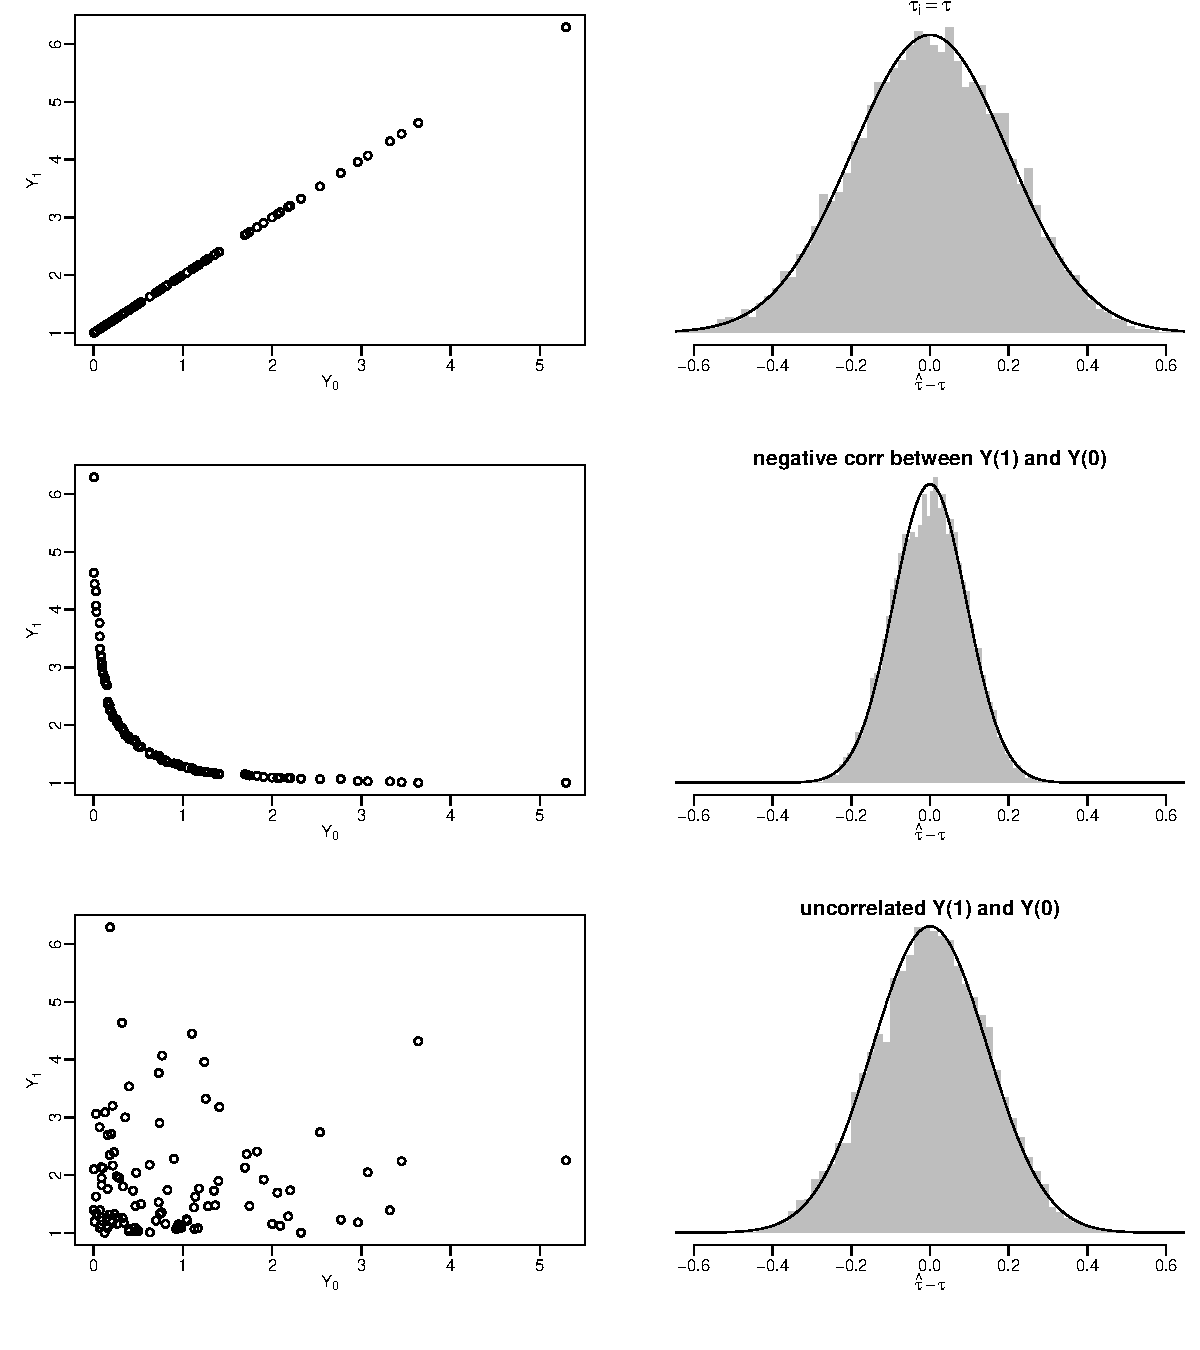
\includegraphics[width = \textwidth]{figures/neymanevaluation3.pdf}
 \caption{
Left: joint distributions of the potential outcomes with the same marginal distributions. 
Right: sampling distribution of $\hat{\tau} - \tau$ over $10^4$ simulations with different joint distributions of the potential outcomes.}\label{fig::simulation-neyman}
 \end{figure} 
 
 
 
 
 
 \subsection{Heavy-tailed outcome and failure of Normal approximations}


The  CLT of $\hat{\tau}  $ in Theorem \ref{thm::clt-difference-in-means} holds under some regularity conditions. Those conditions will be violated with heavy-tailed potential outcomes. We can modify the above simulation studies to illustrate this point. Assume the individual causal effects are constant but the control potential outcomes are contaminated by a Cauchy component with probability $0.1, 0.3$, or $0.5$. The following code generates the potential outcomes with the probability of contamination being $0.1$. 

\begin{lstlisting}
eps = rbinom(n, 1, 0.1)
y0 = (1 - eps)*rexp(n) + eps*rcauchy(n)
y1 = y0 + 1
\end{lstlisting} 


Figures \ref{fig::simulation-neyman-heavytail-1} and \ref{fig::simulation-neyman-heavytail-2} show two realizations of the histograms of $\hat{\tau} - \tau$ with the corresponding Normal approximations. With heavy-tailed potential outcomes, the Normal approximations are quite poor. Moreover, unlike Figure \ref{fig::simulation-neyman}, the histograms are quite sensitive to the random seed of the simulation. 


 \begin{figure}
 \centering 
 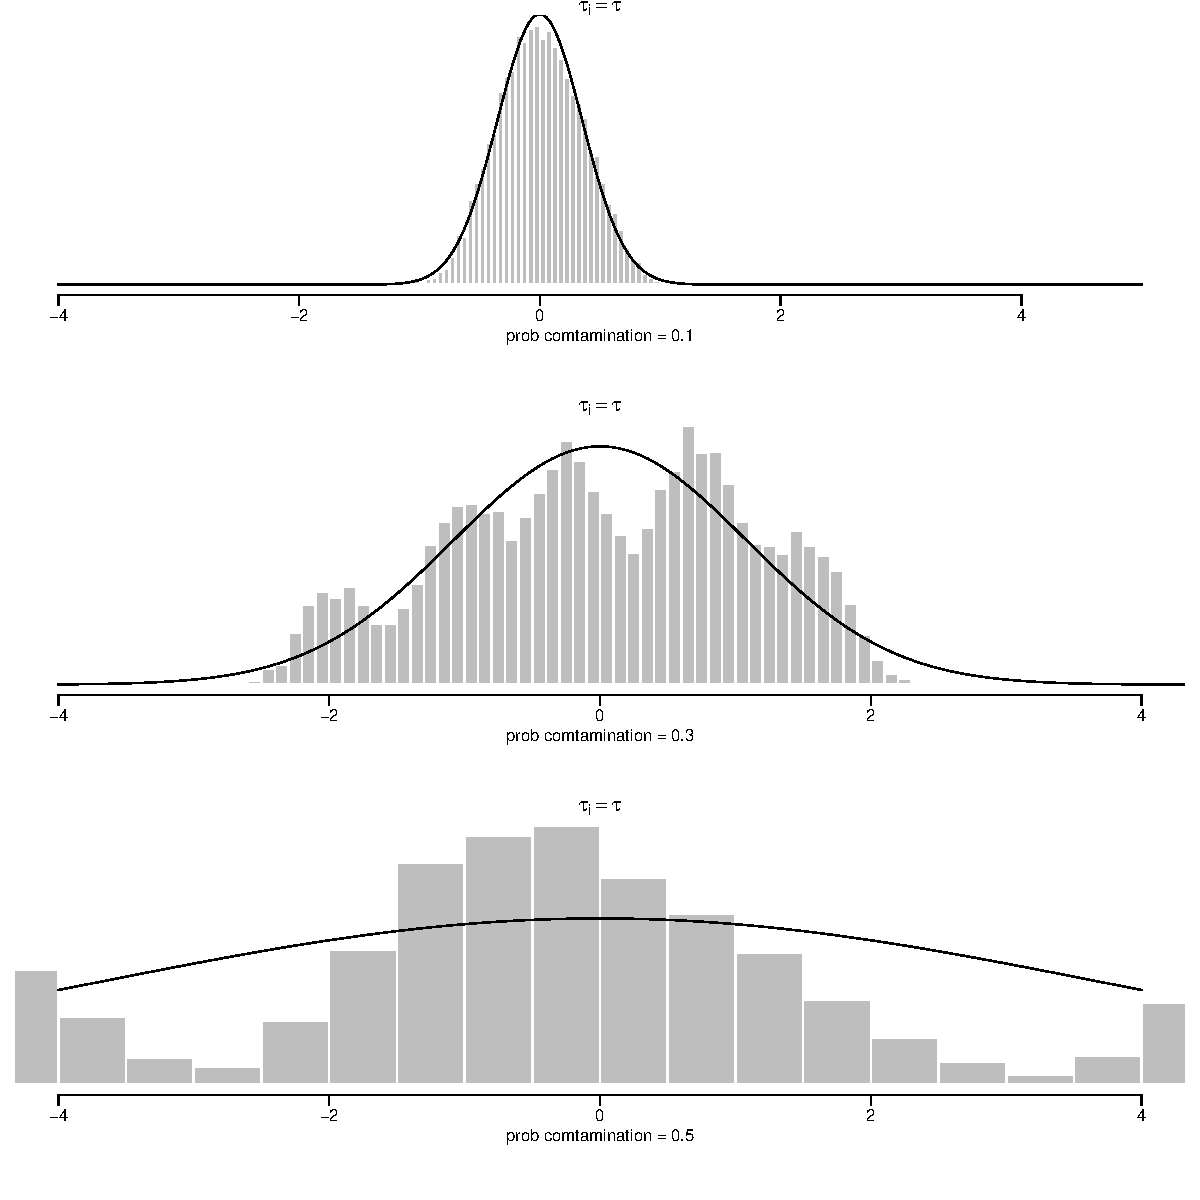
\includegraphics[width = \textwidth]{figures/neyman_comtamination_realized1.pdf}
 \caption{Sampling distribution of $\hat{\tau} - \tau$ with contaminated potential outcomes (with different contamination probabilities): realization one }\label{fig::simulation-neyman-heavytail-1}
 \end{figure} 
 
  \begin{figure}
 \centering 
 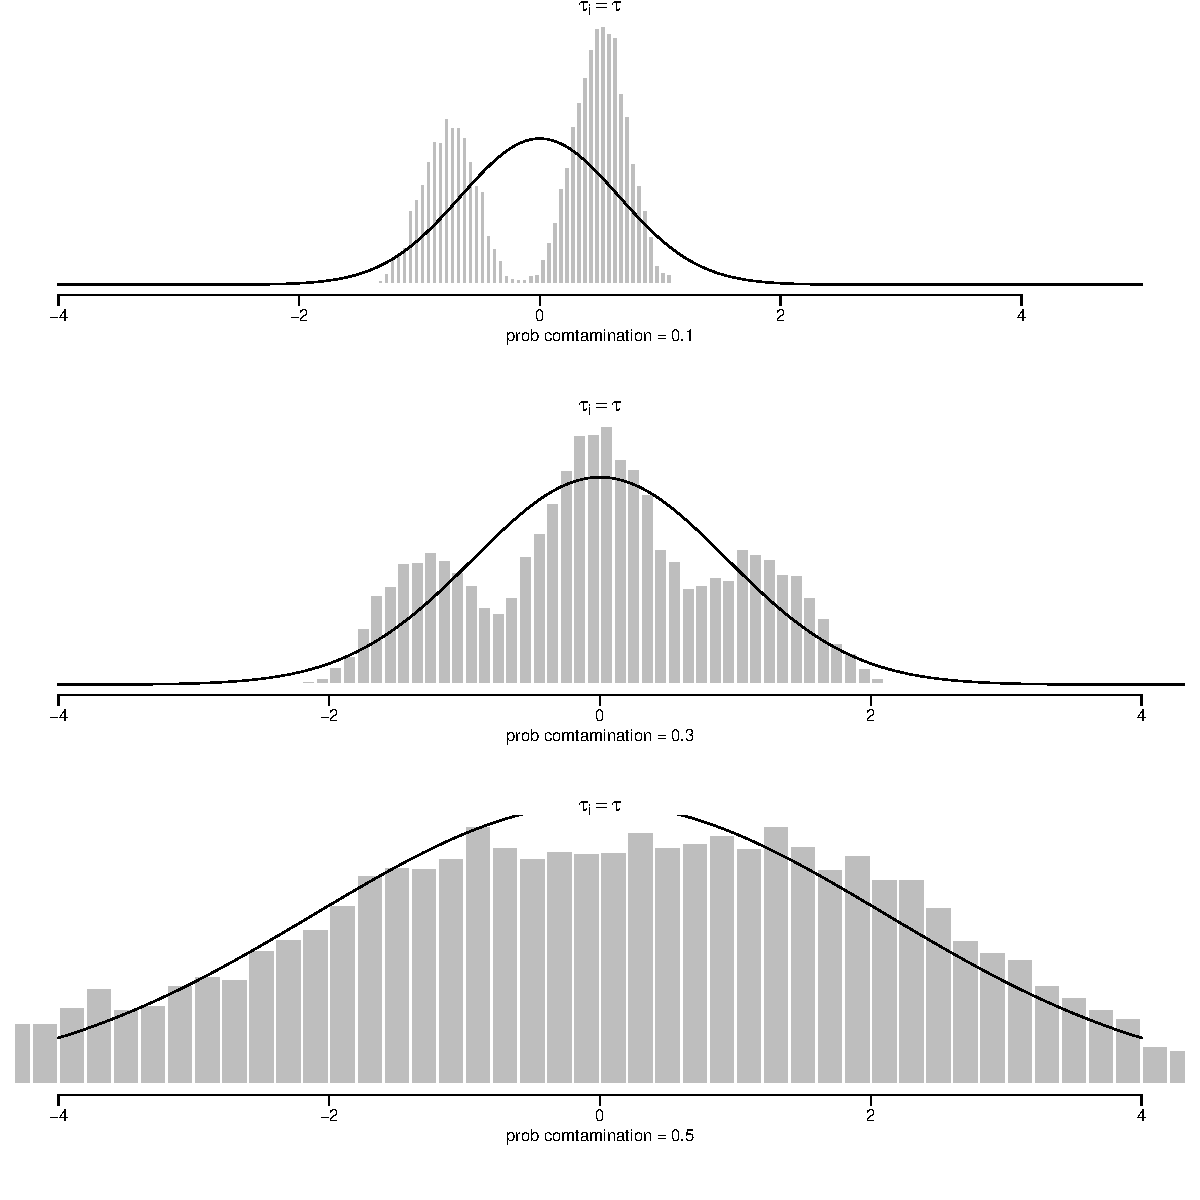
\includegraphics[width = \textwidth]{figures/neyman_comtamination_realized2.pdf}
 \caption{Sampling distribution of $\hat{\tau} - \tau$ with contaminated potential outcomes (with different contamination probabilities): realization two }\label{fig::simulation-neyman-heavytail-2}
 \end{figure} 
 
 


\subsection{Application}
\label{sec::example-neyman-formula}


I analyzed the \ri{lalonde} data in Chapter \ref{sec::frt-lalonde-experiment} to illustrate the idea of the FRT. Now I use the data to illustrate the theory in this chapter. 
\begin{lstlisting}
> library(Matching)
> data(lalonde)
> z = lalonde$treat
> y = lalonde$re78
\end{lstlisting} 

We can easily calculate the point estimator and standard error based on the formulas in Theorem \ref{thm::neyman1923}:
\begin{lstlisting}
> n1= sum(z)
> n0= length(z) - n1
> tauhat = mean(y[z==1]) - mean(y[z==0])
> vhat   = var(y[z==1])/n1 + var(y[z==0])/n0
> sehat  = sqrt(vhat)
> tauhat
[1] 1794.343
> sehat
[1] 670.9967
\end{lstlisting} 

Practitioners often use OLS to estimate the average causal effect which also gives a standard error. 
\begin{lstlisting}
> olsfit = lm(y ~ z)
> summary(olsfit)$coef[2, 1: 2]
  Estimate Std. Error 
 1794.3431   632.8536 
 \end{lstlisting} 
However, the above standard error seems too small compared to the one based on  Theorem \ref{thm::neyman1923}.  This can be solved by using the EHW robust standard error. 
\begin{lstlisting}
> library(car)
> sqrt(hccm(olsfit)[2, 2])
[1] 672.6823
> sqrt(hccm(olsfit, type = "hc0")[2, 2])
[1] 669.3155
> sqrt(hccm(olsfit, type = "hc2")[2, 2])
[1] 670.9967
 \end{lstlisting} 





\section{Homework Problems}

\paragraph{Proof of Lemma \ref{lemma::variancecovariancetau}}\label{hw::proof-covariance-basic}


Prove Lemma \ref{lemma::variancecovariancetau}. 


\paragraph{Alternative proof of Theorem \ref{thm::neyman1923}}\label{hw::neyman-alternative-proof}


Under a CRE, calculate 
$$
\var\{  \hat{\bar{Y}}(1)  \} ,\quad
\var\{  \hat{\bar{Y}}(0)  \} ,\quad
\cov\{  \hat{\bar{Y}}(1) ,  \hat{\bar{Y}}(0)  \} 
$$
and use these formulas to calculate $\var(\hat{\tau} )$. 

Remark: Use the results in Chapter \ref{chapter::SRS-appendix}. 





\paragraph{Neymanian inference and OLS}
\label{hw::neyman-ols-nox}


Prove \eqref{eq::ols-difference-in-means}--\eqref{eq::ols-ehw}. Moreover, prove that the HC2 variant of the EHW robust variance estimator recovers $\hat{V}$ exactly. 

Remark: Chapter \ref{appendix::basic-linear-regression} reviews some important technical results about OLS.
 
 



\paragraph{Treatment effect heterogeneity}\label{hw::treatment-effect-heterogeneity-neyman}


Show that $S^2(\tau) = 0$ implies that $S^2(1) = S^2(0)$. Given a counterexample with $S^2(1) = S^2(0)$ but $S^2(\tau) \neq  0$. 


Show that $S^2(1) < S^2(0)$ implies that 
$$
S(Y(0),\tau)  = (n-1)^{-1} \sumn \{ Y_i(0)  - \bar{Y}(0) \} (\tau_i - \tau) <0.
$$
Give a counterexample with $S^2(1) > S^2(0)$ but $S(Y(0),\tau)  < 0 .$



Remark: The first result states that no treatment effect heterogeneity implies equal variances in the treated and control potential outcomes. But the converse is not true. The second result states that if the treated potential outcome has a smaller variance than the control potential outcome, then the individual treatment effect is negatively correlated with the control potential outcome. But the converse is not true. \citet[][page 293]{gerber2012field} and \citet[][Appendix B.3]{ding2019decomposing} gave related discussions. 



\paragraph{A better bound of the variance formula}
\label{hw::better-bound-neyman}


\cite{Neyman:1923}'s conservative variance estimator essentially uses the following upper bound on the true variance:
$$
\var(\widehat{\tau}) = \frac{S^2(1)}{n_1} + \frac{S^2(0)}{n_0} - \frac{S^2(\tau)}{n} \leq \frac{S^2(1)}{n_1} + \frac{S^2(0)}{n_0},
$$
which uses the trivial fact that $S^2(\tau) \geq 0$. 
Show the following upper bound
\begin{eqnarray}\label{hw::cs-bound-neyman}
\var(\widehat{\tau})  \leq   \frac{1}{n} \left\{   \sqrt{  \frac{n_0}{n_1}  } S(1) +  \sqrt{  \frac{n_1}{n_0}  } S(0)   \right\}^2.
\end{eqnarray}
When does the equality in \eqref{hw::cs-bound-neyman} hold? 

The upper bound \eqref{hw::cs-bound-neyman} motivates another conservative variance estimator 
$$
\hat{V}' =  \frac{1}{n} \left\{   \sqrt{  \frac{n_0}{n_1}  } \hat S(1) +  \sqrt{  \frac{n_1}{n_0}  } \hat S(0)   \right\}^2.
$$
Section \ref{sec::simulation-neyman-formula} used $\hat{V}$ in the simulation. Repeat the simulation with an additional comparison with the variance estimator $\hat{V}' $ and the associated confidence interval. 



Remark: 
You may find Section \ref{sec::cauchy-schwarz-inequality} useful for the proof. 
The upper bound \eqref{hw::cs-bound-neyman} can be further improved. 
\citet{aronow2014sharp} derived the sharp upper bound for $\var(\widehat{\tau}) $ using the Frechet--Hoeffding inequality. Those improvements are rarely used in practice mainly for two reasons. First, they are more complicated than $\hat{V}$ which can be conveniently implemented by OLS. Second, the confidence interval based on  $\hat{V}$ also works under other formulations, for example, under a true linear model of the outcome on the treatment, but those improvements do not. Although they are theoretically interesting, those improvements have little practical impact. 
 


\paragraph{Vector version of \citet{Neyman:1923}} \label{hw::vector-neyman1923}

The classic result of \citet{Neyman:1923} is about a scalar outcome. It is common to have multiple outcomes in practice. Therefore, we now extend the potential outcomes to vectors. We consider the average causal effect on a vector outcome $\bm{V}  \in \mathbb{R}^K$: 
$$
\tau_{\bm{V}} = \frac{1}{n}  \sumn \left\{  \bm{V}_i(1) - \bm{V}_i(0) \right\},
$$
where $\bm{V}_i(1)$ and $\bm{V}_i(0)$ are the potential outcomes of $\bm{V}$ for unit $i$. 
The Neyman-type estimator for $\tau_{\bm{V}}$ is the difference between the sample mean vectors of the observed outcomes under treatment and control:
$$
\widehat{ \tau}_{\bm{V}} = \bar{\bm{V}}_1  - \bar{\bm{V}}_0 
= \frac{1}{n_1}   \sumn Z_i  \bm{V}_i   - \frac{1}{n_0}  \sumn (1-Z_i) \bm{V}_i . 
$$


Consider a CRE. Show that $\widehat{ \tau}_{\bm{V}} $ is unbiased for $\tau_{\bm{V}} $. Find the covariance matrix of $\widehat{ \tau}_{\bm{V}} $. Find a (possibly conservative) estimator for the variance. 


\paragraph{Inference in the BRE}\label{hw::bre-inference}


In this book, I use the following definition for the BRE. 

\begin{definition}
[BRE]\label{def::BRE}
The treatment indicators $Z_i$'s are IID Bernoulli$(\pi)$ with $n_1 = \sumn Z_i$ receiving the treatment and $n_0 = \sumn (1-Z_i)$ receiving the control, respectively. 
\end{definition}



First, we can use the FRT to analyze the BRE. How do we test $\HF$ in the BRE? Can we use the same FRT procedure as in the CRE if the actual experiment is the BRE? If yes, give a justification; if no, explain why.

Second, we can obtain point estimators for $\tau$ and find the associated variance estimators, as \citet{Neyman:1923} did for the CRE. 
\begin{enumerate}
\item
Is $\hat{\tau}$ unbiased for $\tau$? Is it consistent?
\item
Find an unbiased estimator for $\tau$.
\item
Compare the variance of the above unbiased estimator and the asymptotic variance of $\hat{\tau}$. 
\end{enumerate}

Remark: 
Under the BRE, the estimator $\hat{\tau}$ does not have finite variance but the variance of its asymptotic distribution is finite. 



\paragraph{Recommended reading}

 \citet{Ding:2014} compared the Fisherian approach and Neymanian approach to analyzing the CRE. 


